% file: modeledsystems.tex

\chapter{Modeled systems}
The goal of this thesis is to study fracture of methane hydrates. In order to do that, I need to know the mechanical properties of the model I study. Since studies of mechanical properties of methane hydrates modeled with TIP4P/ICE+UAM are scarce, I start this chapter by working out even the basic properties of the model, such as Poissons ratio and Youngs modulus. In order to be sure that the methods I use to estimate the mechanical properties work, I first check them with known values for a Lennard-Jones crystal. 

\section{Shear viscosity and diffusivity of the water model}
I have not been successful in finding values for the shear viscosity and diffusivity of bulk liquid water modeled with TIP4P/ICE. To measure these properties, I run a simulation like the one I ran to calculate verify the same properties for the TIP4P/2005 potential. Figure \ref{fig:viscosity_green_kubo_tip4p_ice} shows the Green-Kubo relation for the viscosity using 5 independent pressure components from 4 indepentent simulations with different simulation box sizes. Based on these data, I estimate the shear viscosity of TIP4P/ICE to $\eta_{GK} = \text{\SI{1.63\pm 0.05}{\milli\pascal\second}}$. 

\begin{figure}
\centering
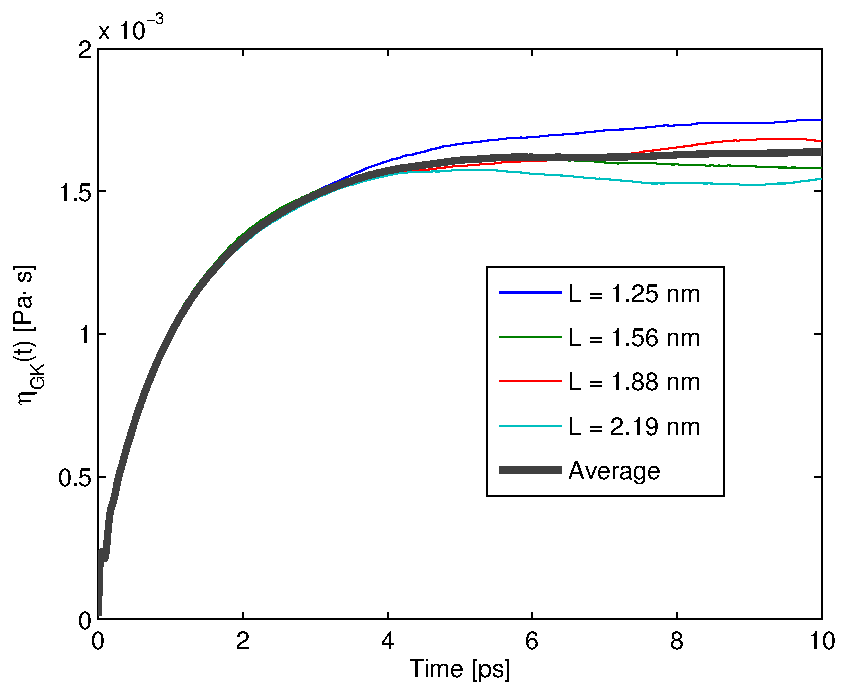
\includegraphics[width=10cm]{../figures/thesis/viscosity_green_kubo_tip4p_ice.pdf}
\caption{Shear viscosity for TIP4P/ICE at \SI{300}{\kelvin} and $\rho = \text{\SI{0.98}{\gram\per\cubic\cm}}$. Each thin line shows the average of the 5 independent pressure component. The thich line is the average of 4 independent simulations. The viscosity is estimated to $\eta_{GK} = \text{\SI{1.63\pm0.05}{\milli\pascal\second}}$}
\label{fig:viscosity_green_kubo_tip4p_ice}
\end{figure}

\begin{figure}
\centering
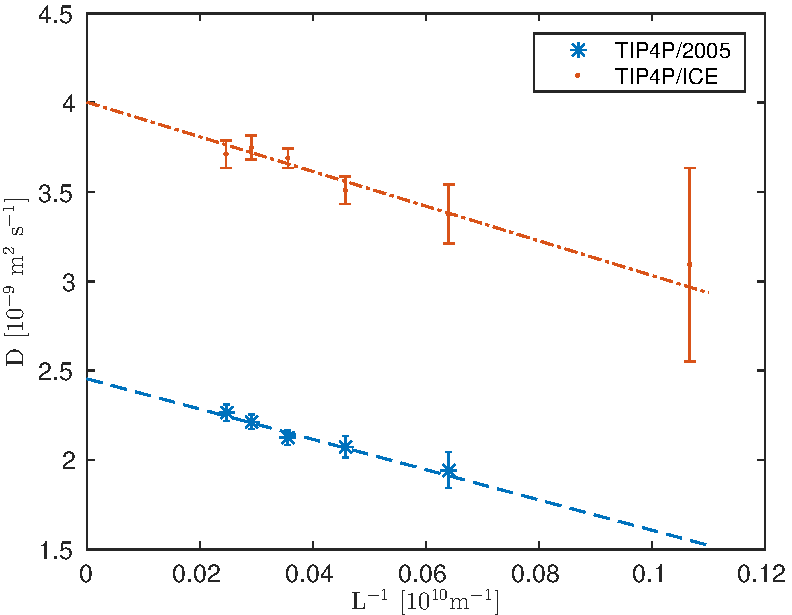
\includegraphics[width=10cm]{../figures/thesis/diffusivity_comparison_tip4p_ice_2005.pdf}
\caption{Linear regression of self diffusion coefficients as a function of inverse simulation box length. Results for TIP4P/2005 (blue) were already reported in the verification section. The self-diffusion coefficient for TIP4P/ICE is estimated to $D_0 = \SI{4.0 \pm 0.1 d-9}{\meter\squared\per\second}$}
\label{fig:diffusivity_comparison_tip4p_ice_2005}
\end{figure}

\section{Measuring elastic properties with a constant strain rate}
A naive approach, which i will use for crude estimates, is to subject a system to a constant strain rate by expanding the simulation box in one of the coordinate directions, and rescale all atom positions accordingly. An anisotropic thermo-barostat should be applied along the other axes, to keep the environment pressure and temperature constant. Since the barostat scales the simulation box, strains along the two axes perpendicular to the applied strain can be measured as the contraction of the simulation box in these directions:

\begin{equation}
\varepsilon_i = \frac{L_i-L_{0, i}}{L_{0, i}}
\end{equation}

If the sample is isotropic, I only have to simulate strain application in one of the coordinate directions to estimate both Young's modulus and Poissons ratio for a given system. To account for the possibility that the model I use do not exhibit isotropic behavior, I will check strains in both of the coordinate axes that are perpendicular to the axis of applied strain when calculating Poissons ratio. The scalar value of $\nu$ is the slope of the strain-strain curve, and for $E$ of the stress-strain curve, both in their linear regions. I will calculate these slopes using linear regression with least squares on the curves.
In the following, I will apply the method described above to a Lennard-Jones crystal and to the TIP4P/ICE+UAM methane hydrate model.

\subsection{Lennard-Jones crystal}
The FCC-lattice with a Lennard-Jones potential has been extensively investigated due to its simplicity. Therefore it provides robust benchmarking capabilities. I want to check that my protocols for dynamic (but quasistatic) determination of elastic properties and fracture strength reproduces known parameters for a Lennard-Jones solid. Reference values are for Young's modulus, $E=61.1 \epsilon/\sigma^3 = \text{\SI{2.40}{\giga\pascal}}$ (for the parameters I use for Methane), and for Poissons ratio, $\nu=0.347$. Values are taken from a molecular dynamics study by Quesnel et al. \cite{Quesnel1993}.

Figures \ref{fig:stress_strain_11_11_11_and_22_22_22_y_z_poisson_lennard_jones} and \ref{fig:strain_strain_11_11_11_and_22_22_22_y_z_poisson_lennard_jones} show data for a strain test of two systems of Lennard-Jones particles subjected to a strain rate of \SI{2d-8}{\per\femto\second} over \SI{0.8}{\nano\second} resulting in a maximum strain of \SI{0.8}{\percent}. The external pressure was set to \SI{50}{\mega\pascal}, and the temperature was \SI{5}{\kelvin}. Along with the data are estimates of Poissons ratio and Young's modulus, taken as the best linear regression with least squares. 


\begin{figure}
\centering
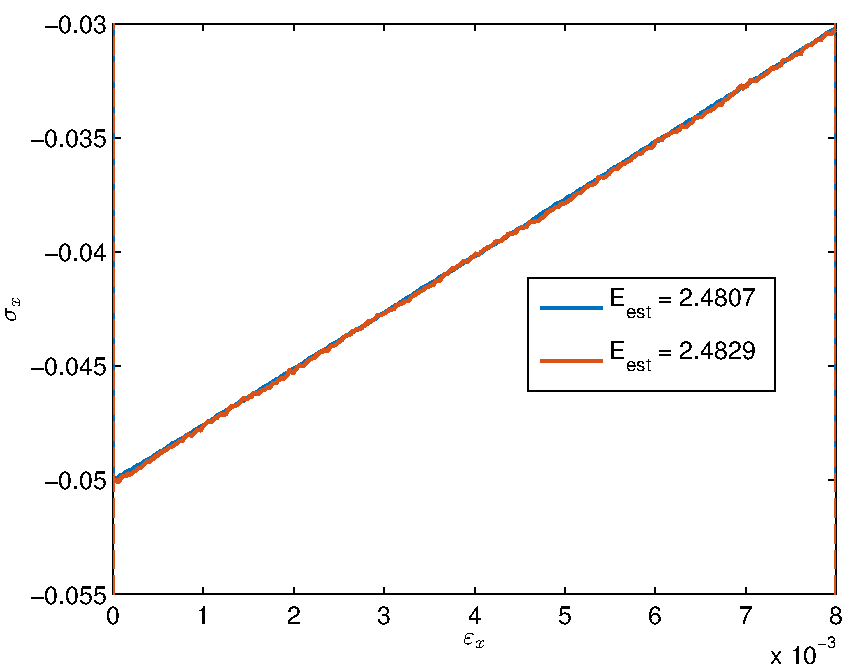
\includegraphics[width=10cm]{../figures/thesis/stress_strain_11_11_11_and_22_22_22_y_z_poisson_lennard_jones.pdf}
\caption{Stress-strain relations for Lennard-Jones systems of $11^3$ (red) and $22^3$ (blue) FCC unit cells. The sample was subjected to a constant strain rate of \SI{2d-8}{\per\femto\second}. $E$ is estimated using linear regression with least squares on all data points.}
\label{fig:stress_strain_11_11_11_and_22_22_22_y_z_poisson_lennard_jones}
% Path to simulation: /media/henriasv/Data/molecular-data/master_methane_hydrates/stress_strain/20150113_lennard_jones_strain
\end{figure}

\begin{figure}
\centering
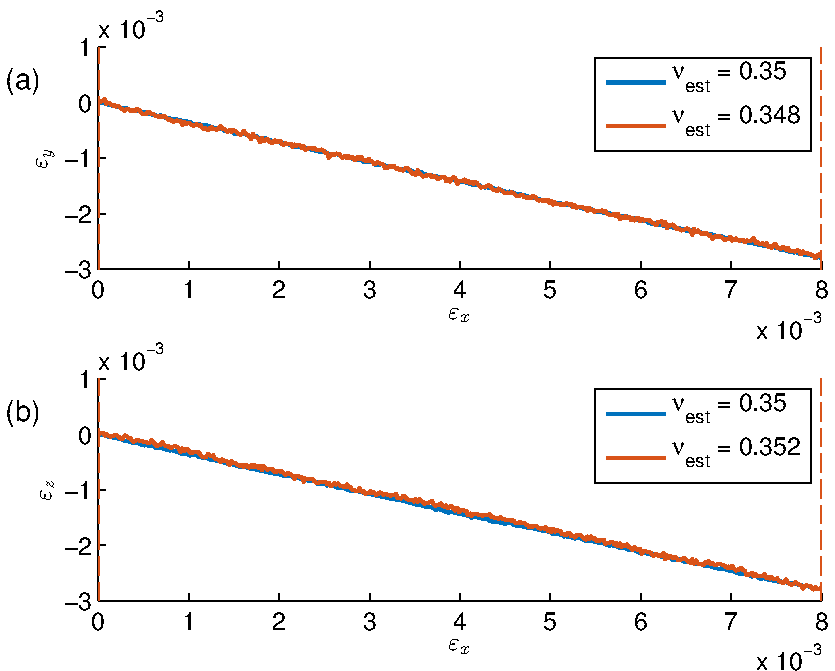
\includegraphics[width=10cm]{../figures/thesis/strain_strain_11_11_11_and_22_22_22_y_z_poisson_lennard_jones.pdf}
\caption{Strain-strain relations for for the same simulations as in Figure \ref{fig:stress_strain_11_11_11_and_22_22_22_y_z_poisson_lennard_jones}. All data points were used to estimate $\nu$.}
\label{fig:strain_strain_11_11_11_and_22_22_22_y_z_poisson_lennard_jones}
% Path to simulation: /media/henriasv/Data/molecular-data/master_methane_hydrates/stress_strain/20150113_lennard_jones_strain
\end{figure}

\subsection{S1 methane hydrate with TIP4P/ICE+UAM}
To my knowledge, there are no published estimates of Youngs modulus and Poissons ratio for the TIP4P/ICE+UAM model of methane hydrates. Therefore, I seek to make crude estimates of these quantities in dynamic simulations. I apply a constant strain rate by continously rescaling particle positions in one direction during MD-simulations. The other directions are kept under a constant pressure with anisotropic barostatting.
Figure \ref{fig:stress_strain_11_11_11_tip4p_ice_uam} shows the stress strain relationships and corresponding estimates of Youngs modulus for a system of 11x11x11 S1 unit cells subjected to strain rates of \SI{5d-7}{\per\femto\second} and \SI{2d-7}{\per\femto\second}. By extrapolating the results to quasistatic strain, Youngs modulus is estimated to \SI{7.1}{\giga\pascal}. 
Figure \ref{fig:strain_strain_11_11_11_y_z_poisson_tip4p_ice_uam} shows the relationship between applied strain along the x-axis and the measured strain along the other axes. It is not outrageous to assume S1 methane hydrate to be isotropic. Under this assumption, and by extrapolation to quasisatic strain, I estimate the poisson ratio for this model of S1 methane hydrate to be $\nu = 0.41$. 

\begin{figure}
\centering
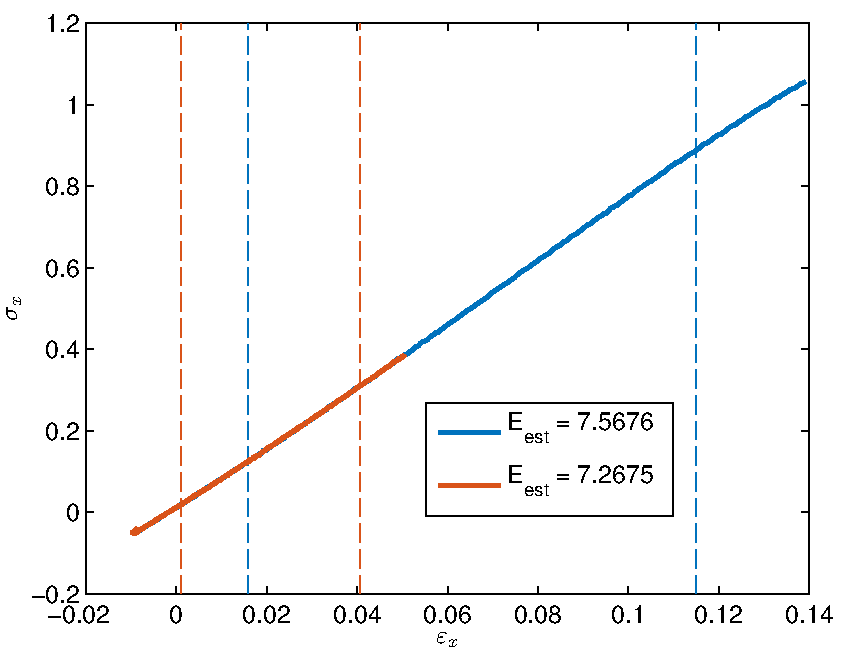
\includegraphics[width=10cm]{../figures/thesis/stress_strain_11_11_11_tip4p_ice_uam.pdf}
\caption{Stess-strain relations for a system of 11x11x11 S1 unit cells. Dashed lines indicate the region that was used to estimate Youngs modulus. Strain rates of \SI{5d-7}{\per\femto\second} (blue) and \SI{2d-7}{\per\femto\second} (red) along the x-axis. Upon close visual inspection, a slight rising slope can be seen for small strains and a rising slope for large strains, but overall the stress-strain relation is suprisingly linear, especially given the large strain-range.}
\label{fig:stress_strain_11_11_11_tip4p_ice_uam}
% Path to simulation: /media/henriasv/Data/molecular-data/master_methane_hydrates/stress_strain/20150108_youngs_modulus

\end{figure}

\begin{figure}
\centering
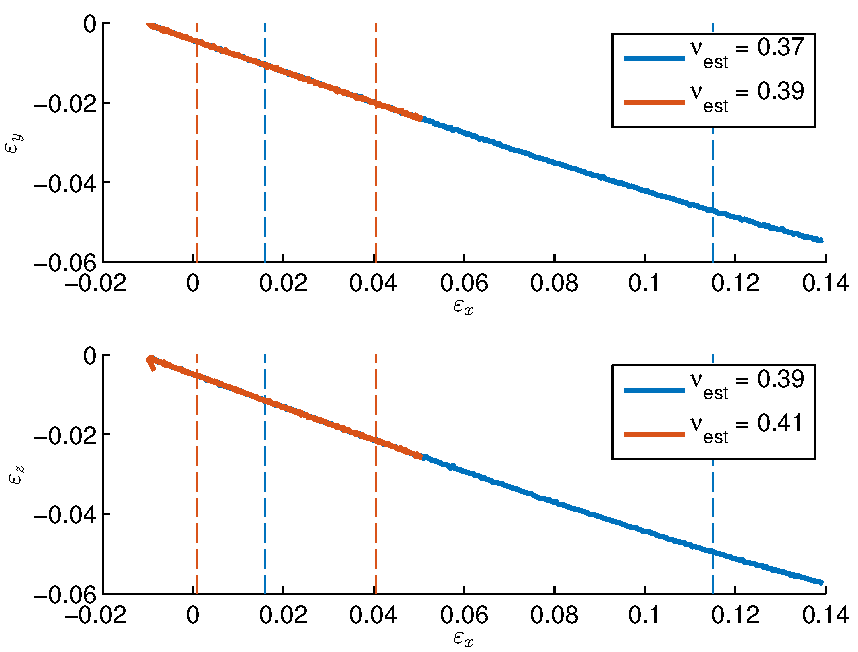
\includegraphics[width=10cm]{../figures/thesis/strain_strain_11_11_11_y_z_poisson_tip4p_ice_uam.pdf}
\caption{Strain-strain relations for the same system as in Figure \ref{fig:stress_strain_11_11_11_tip4p_ice_uam}. Measured strain along the y-axis (a) and z-axis (b) is plotted against the applied strain along the x-axis. Dashed lines indicate the region that was used to estimate Poissons ratio.}
\label{fig:strain_strain_11_11_11_y_z_poisson_tip4p_ice_uam}
% Path to simulation: /media/henriasv/Data/molecular-data/master_methane_hydrates/stress_strain/20150108_youngs_modulus

\end{figure}

\section{Early results on fracture and fracture toughness}

\subsection{Determining the critical stress intensity factor}
As described in the section about fracture mechanics, the stress intensity factor is commonly used to calculate the fracture toughness of a material. The critical energy release rate is usually defined as:
\begin{equation}
	G_C = -\left(\frac{\partial P}{\partial A_{\text{crack}}}\right)_{T, \text{loading}}
	\label{eq:def_critical_energy_release_rate}
\end{equation}

I will follow the method of \cite{Hantal2014} to calculate the critical stress intensity factor (This method was used for illite with ClayFF and ReaxFF):\begin{equation}
	G_C = V \frac{\int_0^{E_{\text{final}}}\uuline{\Sigma}(E) : \dd \uuline{E}}{\int_0^{E_{\text{final}}} \dd A_{crack}}
	\label{eq:hantal_critical_energy_release_rate}
\end{equation}

This is in principle sufficient to determine the critical energy release rate for any mode of loading, provided that the conditions for using Equation \ref{eq:hantal_critical_energy_release_rate} to estimate the critical energy release rate are met.

\subsection{Simulation details}
@VerifyThatThisIsADescriptionOfHantal2014
It is not at all obvious how to perform simulations to determine the fracture toughness. \citet{Hantal2014} performed NVT simulations and imposed a series of small deformations to their sample. After each deformation, they minimized the system, and then ran molecular dynamics for \SI{10}{\pico\second}. I have tried to use the same protocol, but find that for my system, the impact on the energy distribution among the degrees of freedom is too large when performing minimizations between the deformations. this results in a system farther out of equlilibrium that the deformed but not minimized system. Therefore, a possible protocol:

\begin{enumerate}
\item Equilibrate the system NVT (Molecular dynamics)
\item Perform small deformation
\item Reequilibrate the system NVT (Molecular dynamics)
\item If the strain i low: Return to 2. If the strain is high: continue.
\item Molecular dynamics run to wait for failure
\item If failure does not occur, or crack length stabilizes: Return to 2. 
\end{enumerate}

However there are problems here: The waiting time when waiting for failure must be carefully chosen, and if it turns out that critical and sub-critical failure are hard to distinguish, or even impossible to define, then waiting times can be arbitrarly long. 

From the latter discussion, I propose to exploit the possible time problem, and investigate the dependence on strain and temperature on the crack velocity and the waiting time before fracture occurs. The latter is possibly computationally expensive to get sufficient statistic to make any confident statements. 

A simpler protocol -- and I believe this to be a good way to study this particular system -- is to subject the sample to a constant strain rate, then wait for a crack to propagate. This is simple to do, and is also close to experimental conditions. The downside is that the loading is varying during fracture, disturbing measurements of properties like crack velocity at constant loading. It is, however, reasonable to believe that at low strain rates, these effects will be small, if not negligible. This can also be solved by setting the strain rate to zero at some predefined strain level, which is estimated from experience, and can be systematically varied. 


\subsection{Proof-of-concept simulations}
Before performing serious simulations, I do preliminary simulations to find out whether the protocol proposed in the latter section can produce interesting results. I do simulations on a relatively small and quasi 2-dimensional system -- the system is only one unit cell thick -- to keep computational costs down. The total computational cost for tuning in on parameters and getting rid of bugs and blunders was about $10^4$ cpu hours.

Figure \ref{fig:proof_of_concept_crack} shows the potential energy and strain for four simulations where S1 methane hydrates of 24x24x1 unit cells were gradually subjected to a strain of between 0.045 and 0.1 (see figure caption for simulation details). Then, the system was left on its own. For three of the systems, a crack started propagating, for two of them after the strain rate was set to zero. Using the change of internal energy from before to after crack propagation as an estimate of the surface energy, and the area of the box face parallell to the crack as an estimate of the crack area, I can estimate the critical energy release rate. I can also use the change in energy from the initial thermalized system to the split system after crack propagation to estimate the surface energy. Whatever energy change $\Delta U$ I use, the formulas for $G_c$ and $\gamma_s$ reads:

\begin{equation}
	G_c \approx \frac{\Delta U}{L_yL_z}
\end{equation}

\begin{equation}
	\gamma_s \approx \frac{\Delta U}{2 L_y L_z}
\end{equation}

Where the $\frac{1}{2}$ factor is because the crack opens two surfaces. The thermalization for all four of the simulations are equal, with an average potential energy of $\SI{-2.8112}{\femto\joule}$ on the plateau (40--100 \si{\pico\second}). The average potential energy after crack propagation was $\SI{-2.7970}{\femto\joule}$, with almost no variation among the simulations. This yields an energy difference of \SI{1.42d-17}{\joule}. Using the simulation box side face area (measured values: $L_y = \SI{288.8}{\angstrom}$, $L_z = \SI{12.04}{\angstrom}$) as an estimate of the crack size, I get an estimated surface energy of $\gamma_s = \SI{0.204}{\joule\per\meter\squared}.$
@FindFractureToughnessFromGammaAndFromMaxEnergy

\begin{figure}
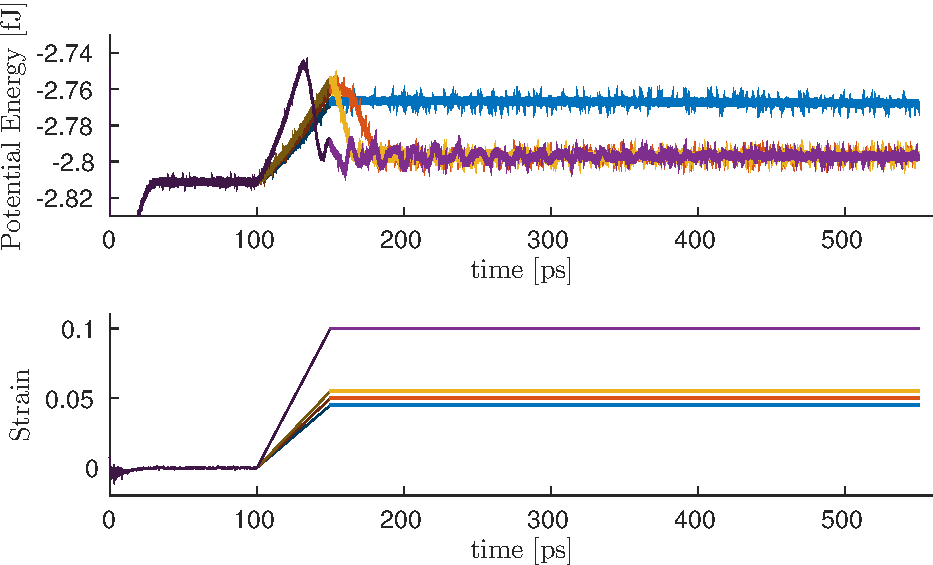
\includegraphics[width=\textwidth]{../figures/thesis/proof_of_concept_poteng_strain.pdf}
\caption{Potential energy (upper panel) and strain (lower panel) for a series of simulations where systems of 24x24x1 unit cells S1 hydrate are subjected to tensile strain. The systems were initiated with an elliptic crack of $6.0 \times 40.0 \si{\angstrom}$. The system was allowed to equilibrate NPT during \SI{100}{\pico\second}, which can be seen from the small fluctuations in strain in this timeframe. Then the simulations were NVT, but with imposed volume change due to the application of a constant strain rate, taking the system to a predesignated stress after \SI{50}{\pico\second}. Then, a regular NVT-simulation was run for \SI{400}{\pico\second} (bright colors). The thermostat and barostat damping times were \SI{1000}{\pico\second}. $T=\SI{260}{\kelvin}$. Falling potential energies correspond to crack opening (in these specific simulations). The slope of falling potential energy is systematically steeper for higher values of the strain before crack propagation. The systems that crack show oscillating potential energy after crack propagation, which is due to global oscillations of the system. The oscillations are damped out by a drag term in the thermostat. }
\label{fig:proof_of_concept_crack}
\end{figure}

\paragraph{Detailed crack analysis}
This is the point at which I developed my code to measure the crack area. Hopefully, that estimate will be better than the estimate solely based on the simulation box dimensions. The code also lets me follow the crack area in time, which makes it possible to measure the crack speed. I choose to define the crack speed as the change of crack area divided by the crack width, since the crack width is well defined – it is $L_z$ of the simulation box. Keeping in mind that my cracks travel in two directions, the crack velocity for a crack initiated as a hole parallell to the z-axis is:

\begin{equation}
v_c = \frac{1}{2L_z}\frac{\dd A_c}{\dd t}
\end{equation}

@MeasureCrackInTimeForTheseSimulations

\paragraph{Summary of concept simulations} The results from this initial simulation indicate that methane hydrate under these conditions are very brittle on the tens-of-picoseconds scale, in the sense that they do not at all plastcally deform to withstand strain. They either deform elastically, or they fail. There is also indications that the time before fracture depends on the applied strain in a systematic way. A close look at the potential energy curve of the simulation in figure \ref{fig:proof_of_concept_crack} that did not end in rupture reveals that the potential energy is actually slowly decreasing. Whether this is a sign of a coming fracture, strengthening rearrangements of particles -- which could imply some ductility -- or something else, remains to be investigated. 

\subsection{Arising questions}
Several quiestion arise as a result of the proof-of-concept runs:
\begin{itemize}
\item Is there a relationship between the waiting time from straining ends till rupture starts and the slope of the potential energy curve?
\item Is the slowly decreasing potential energy of long waiting-time events important, and can it be realted to the waiting time?
\item What is the fracture toughness for long (infinite) waiting times, and is it possible to measure? Will the system melt before it fractures?
\end{itemize}

There are also several technical problems that can be addressed:
\begin{itemize}
\item What is the effect of the thermostat damping time on fracture properties?
\item Is the strain rate important? Does the time it takes to strain the system compete with the waiting time until fracture?
\end{itemize}


\section{Energy considerations -- the thermodynamics of expanding the simulation box}
In the last section, I only considered the potential energy to estimate the fracture toughness, since fracture mechanics dictates that the fracture toughness should be the amount of potential energy released per projected crack surface area opened. In this section, I argue that it is the Helmholtz free energy release rate that should be used for fracture toughness calculations. This solves the problem of methane hydrate fracture seeming very brittle while having $\mathcal{G}_c > 2\gamma_s$.

Let's consider expanding the simulation box along the x-axis. This corresponds to perform work on the system:

\begin{equation}
	W = \int_{t(L_x = L_x^0)}^{t(L_x^0 + \Delta x)} \int_{yz} \sigma_{xx} (t, y, z) \ \dd z \dd y \dd x
\end{equation}

If the system is in equilibrium, then:
\begin{equation}
\int_{yz} \sigma_{xx} (t, y, z) \ \dd z \dd y = L_yL_z\Sigma_{xx}(t)	
\end{equation}
Where $\Sigma_{xx}$ is an element of $\uuline \Sigma$, which is the mean stress tensor for particles in the system. The work on the system can then be written:

\begin{equation}
	W = L_y L_z \int_{t(L_x = L_x^0)}^{t(L_x^0 + \Delta x)} \Sigma_{xx}(t) \ \dd x
\end{equation}
This expression can easily be extracted from a molecular dynamics simulation.
In the canonical ensemble (NVT), the change of internal energy will be:
\begin{equation}
	\Delta U = W + T\Delta S
\end{equation}
When expanding the system, the entropy per temperature will increase, as more microstates are available. This has to be compensated by adding heat. In molecular dynamics, the thermostat effectively adds energy as entropy during simulation box expansion. Furtermore, this energy cannot increase the kinetic energy, since N and T are kept fixed, so all the added heat must be absorbed as potential energy. This means that expanding the simulation box adds a lot of potential energy to the system, both directly through mechanical work, and indirectly through heat. The mechanical work is stored as positional energy -- particles are positioned higher in each others potentials. The heat absorption is more subtle: The system creates more available microstates when it expands homogeneously at a constant temperature. These microstates do only exist because of the strained state of the system, and will disappear if the strain disappears, for example during fracture. The entropy energy is not available for mechanical work. This is why Helmholtz free energy should be considered:

\begin{equation}
	F = U - TS
\end{equation}

This is exactly the energy available for mechanical work. The reason for this tedious discussion of expanding a box is that Helmholtz free energy is not directly available from molecular dynamics simulations. The change in Helmholtz free energy must be explicitly done by integrating the stress tensor of the system. When analyzing fracture, it would be tempting to use the change in total energy or potential energy to estimate the fracture toughness. But this would be wrong -- the fracture toughness should be caclculated using the available mechanical energy. The energy release rate is the amount of Helmholtz free enegry needed to create projected crack surface area, not the change in potential or total energy of the system during fracture. This distinction is not easy to see when reading fracture mechanics, as fracture mechanics usually deal with elastic bodies with no temperature, but it is crucial when studying fracture in molecular dynamics.

When the crack propagates, the stress in the solid methane hydtate is released, and the system consists of a piece of solig methane hydrate and some free gas in between. We don't know the entropy of this system, but it seems reasonable from the strain energy compared to the potential energy that the change in entropy from before straining to after fracture is small compared to the strain energy -- unless, of course, the system was strained significantly more than necessary.


\section{Large simulations of fracture}
\subsection{Complete analysis of a single simulation}
In this subsection, I present analysis results from using all the tools that were presented in the tools section. I analyze a single simulation, but the analyzes here will be representative of how I measure properties that will show up in later results where data from several simulations are used together to say something more general.

\begin{framed} 
\textbf{Simulation details:} A system consisting of $24 \times 24\times 12$ S1 unit cells was prepared. First, an elliptical hole in the xy-plane spanning the whole z-direction was carved out as described in section \ref{subsec:reg_eprism}. The system was then allowed to equilibrate with an anisotropic NPT thermo-barostat for \SI{100}{\pico\second}, with ambient barostat pressure (\SI{101325}{\pascal}). The system was then integrated NVT and subjected to a constant strain rate taking it to a strain level of 0.048 after \SI{50}{\pico\second}. Then straining stopped, and the system was left NVT for \SI{350}{\pico\second}. The damping time of the thermostat and barostat during the whole simulations was $t_{damp} = \SI{1}{\ps}$. The thermostat temperature was \SI{260}{\kelvin}.
\end{framed}


\begin{figure}
\begin{minipage}[b]{0.5\linewidth}
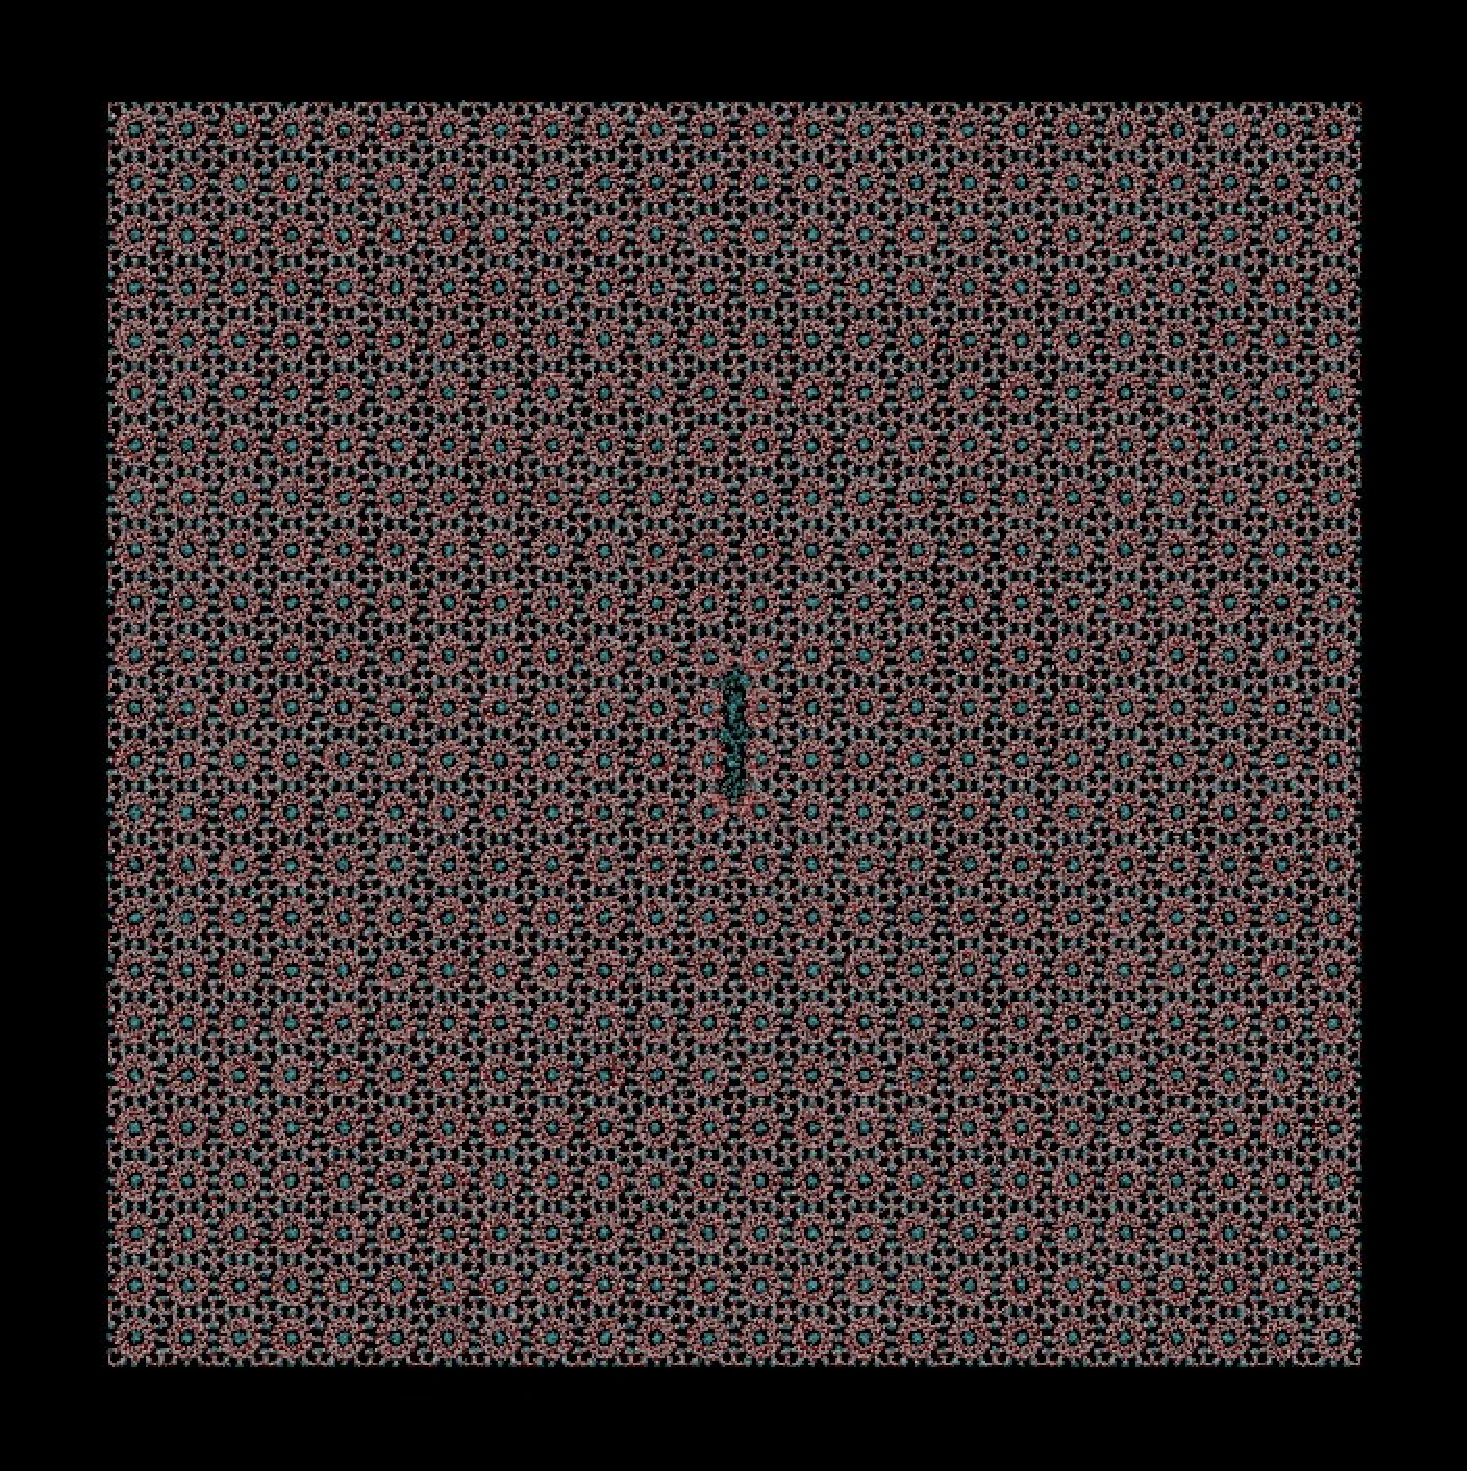
\includegraphics[width=\textwidth]{../snapshots/c_1.pdf}
\end{minipage}
\begin{minipage}[b]{0.5\linewidth}
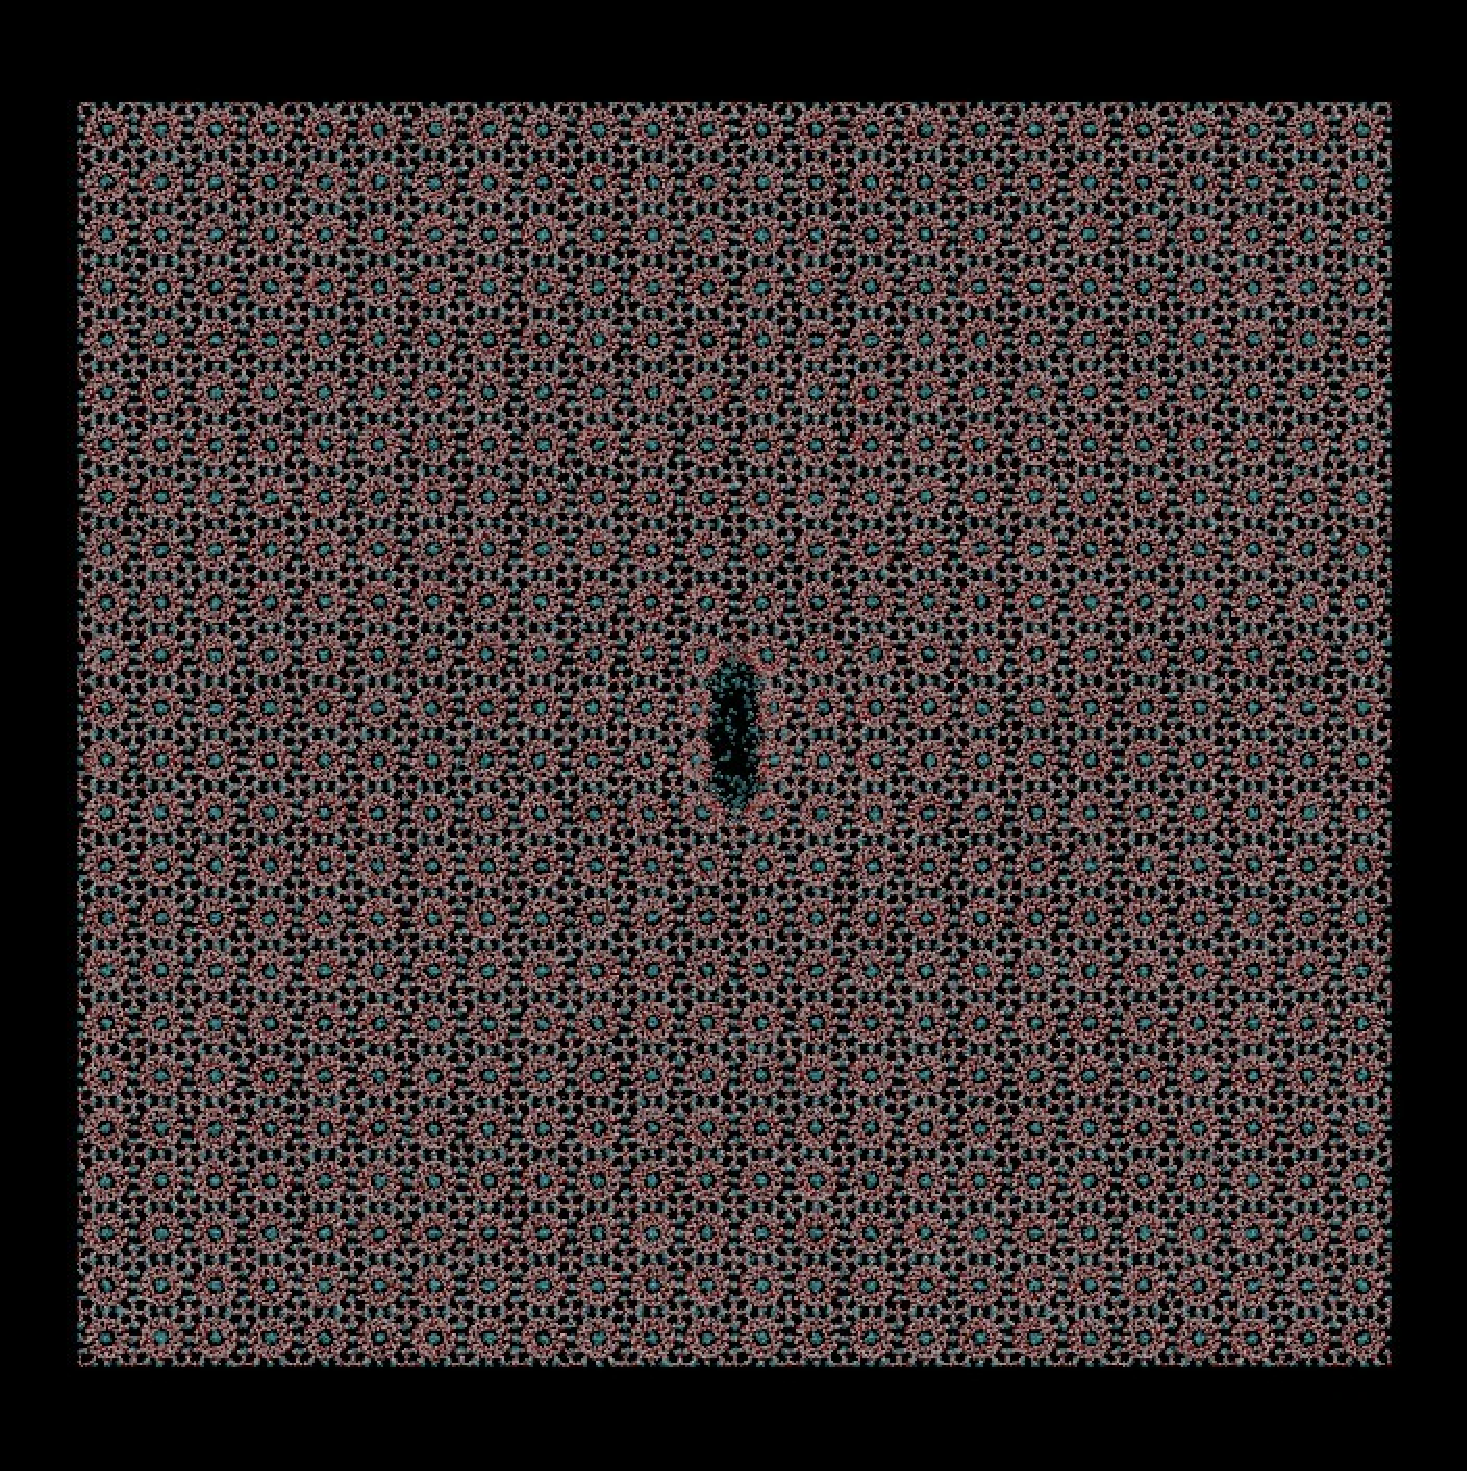
\includegraphics[width=\textwidth]{../snapshots/c_2.pdf}
\end{minipage}
\begin{minipage}[b]{0.5\linewidth}
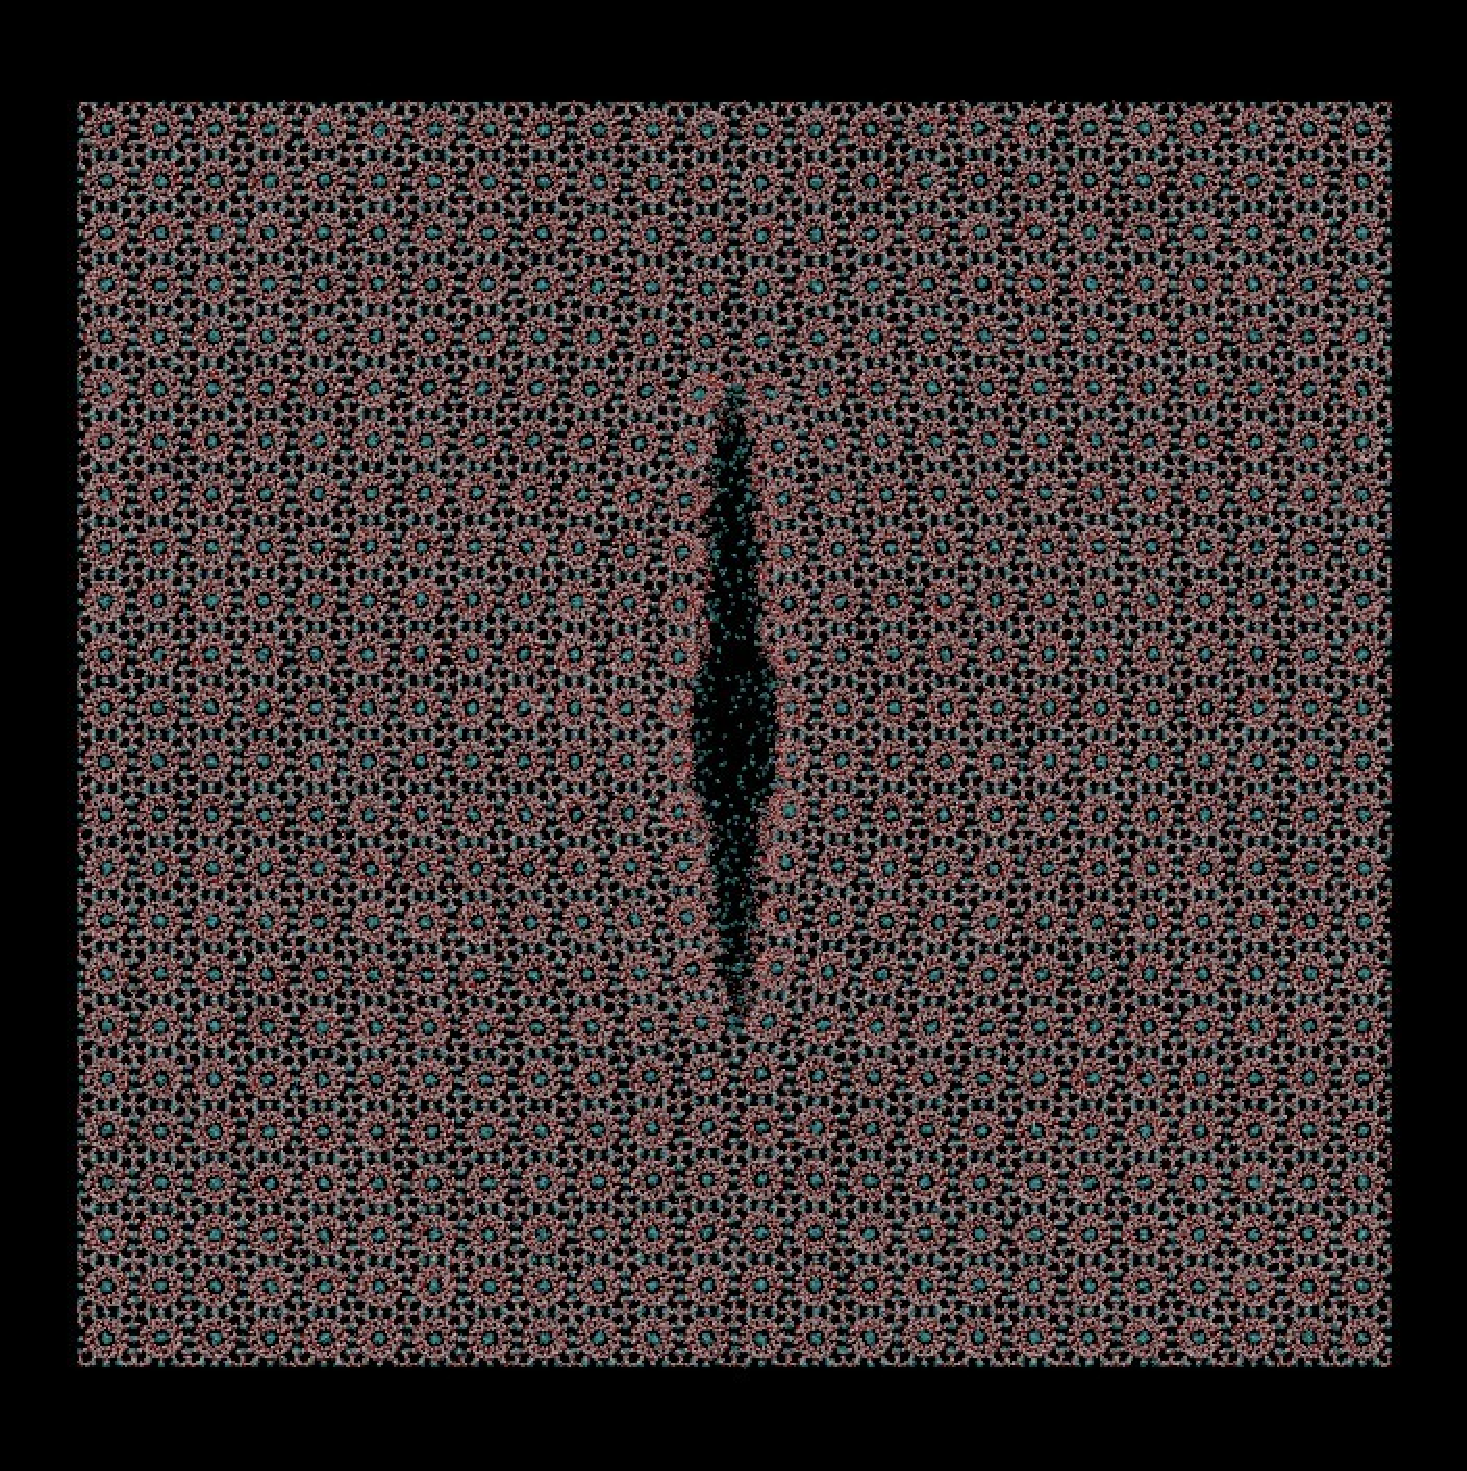
\includegraphics[width=\textwidth]{../snapshots/c_3.pdf}
\end{minipage}
\begin{minipage}[b]{0.5\linewidth}
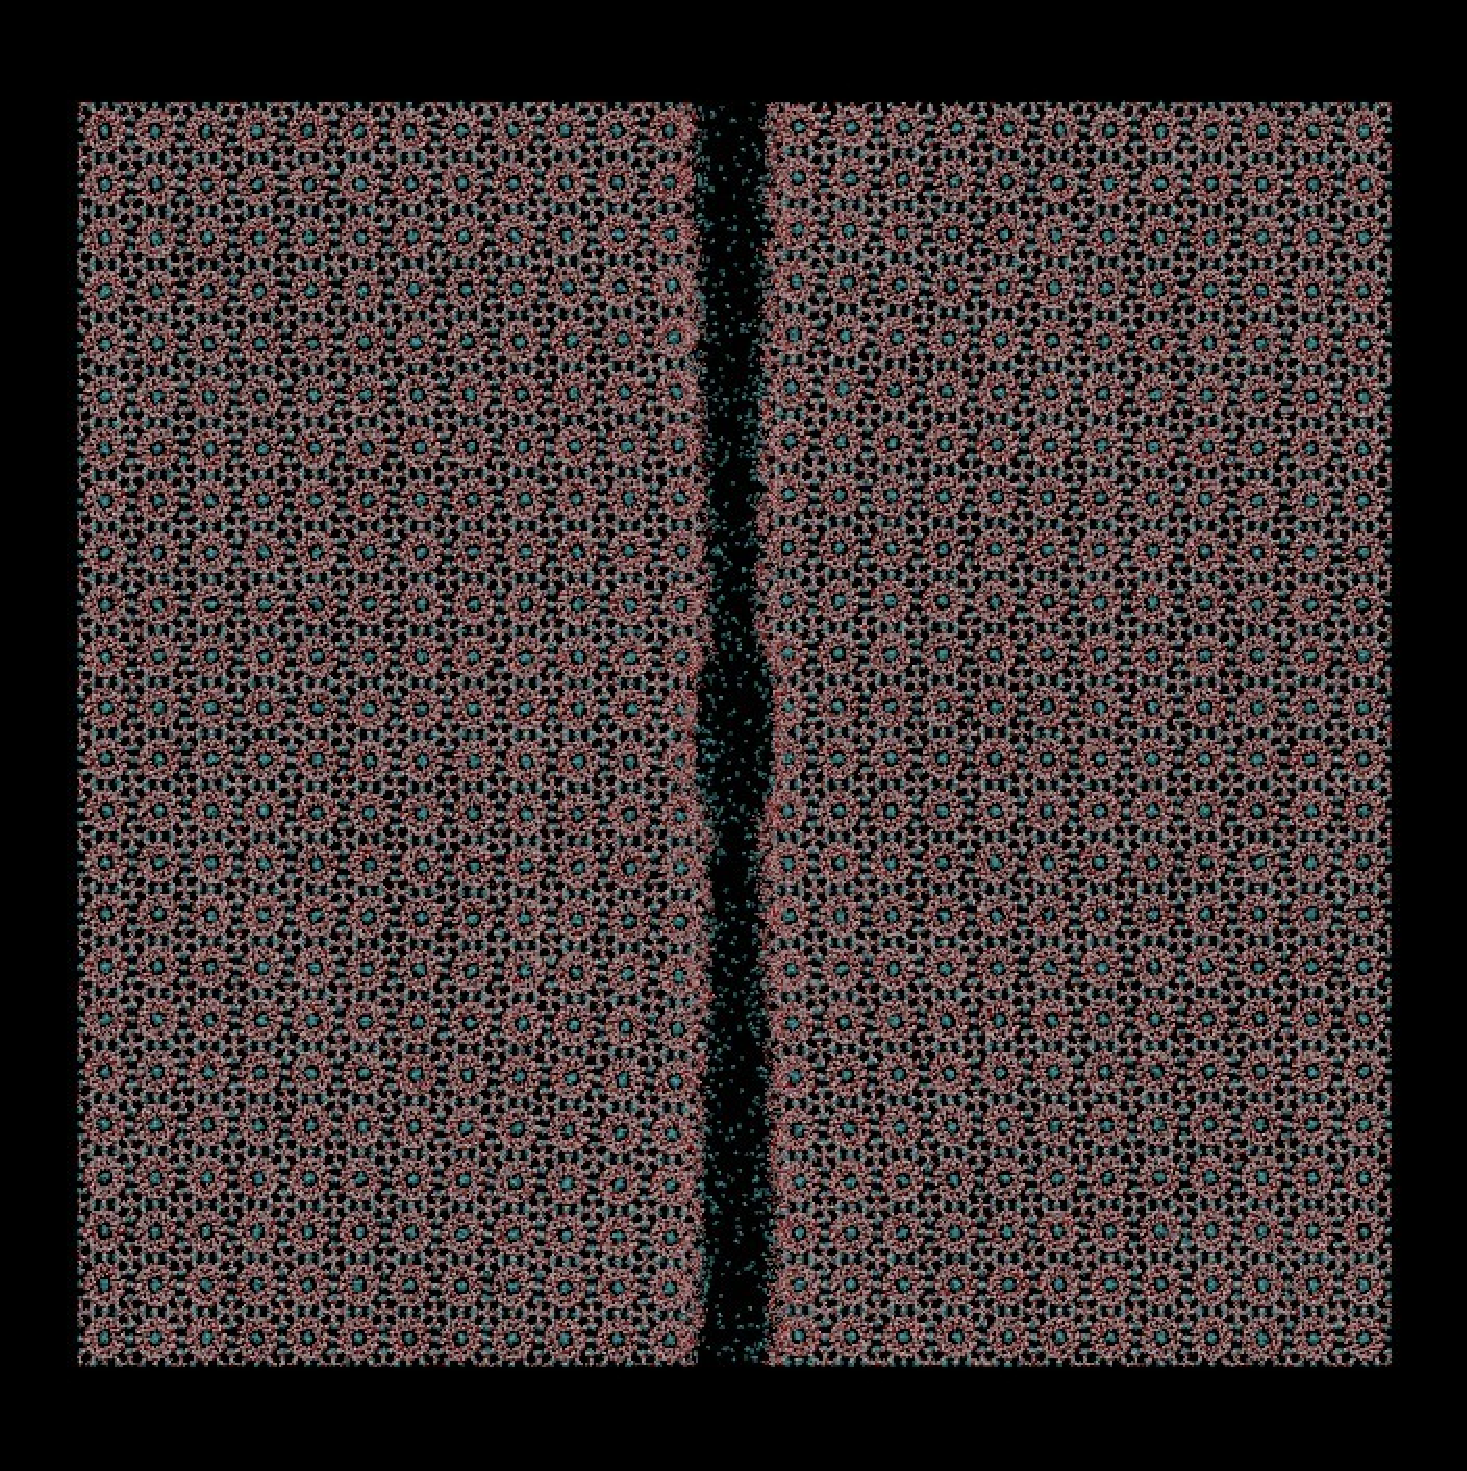
\includegraphics[width=\textwidth]{../snapshots/c_4.pdf}
\end{minipage}
\caption{(upper left) Equilibrated system, \SI{90}{\pico\second}. (upper right) Fully strained system ($\varepsilon_{xx} = 0.048$), \SI{150}{\pico\second}. (lower left) Crack started propagating, \SI{180}{\pico\second}. (lower right) Crack fully propagated after \SI{210}{\pico\second}. The crack is wider near the xz-plane periodic boundary at this point in time due to global oscillations following the crack propagation.}
\end{figure}

Figure \ref{fig:stressfield_avg_wait_for_crack} shows all components of the stress tensor of the system. 

\begin{figure}
\centering
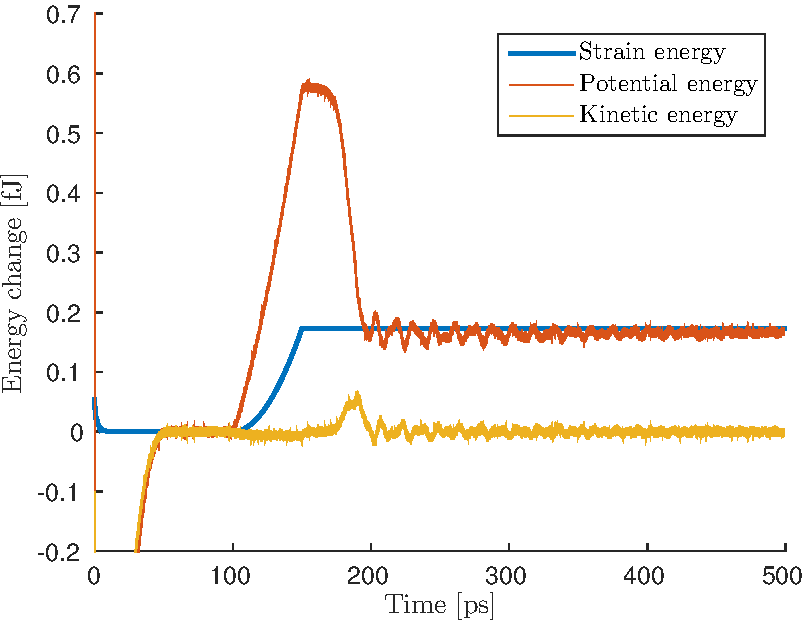
\includegraphics[width=10cm]{../figures/thesis/strain_pot_kin_eng_1048_24_24_12.pdf}
\caption{Strain energy, potential energy and kinetic energy for the whole 0.048 strain simulation. The values are rebased at $t=\SI{100}{\pico\second}$ where straining starts. The kinetic energy corresponds to the temperature, and we see that the temperature slightly drops while the strain increases, and increases during crack propagation. The strain energy imposed on the system is just slightly higher than the energy difference between the unstrained system and the fractured system.}
\end{figure}



\begin{figure}
\centering
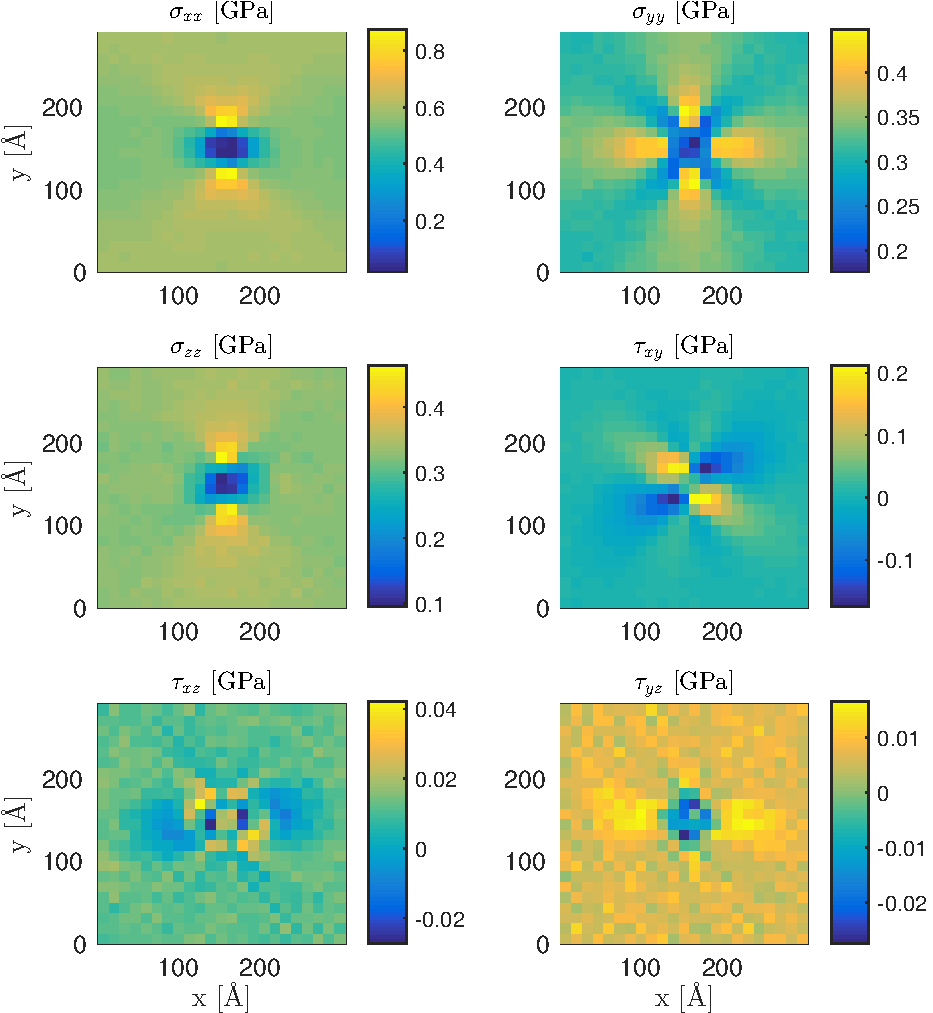
\includegraphics[width=\textwidth]{../figures/thesis/stressfield_avg_wait_for_crack.pdf}
\caption{Stess field averaged over \SI{20}{\pico\second} just after straining was stopped, and while waiting for a crack to start. The modeled system is $24\times 24\times 12$ S1 unit cells. The four uppermost panels show features qualitatively in line with the analytical solution of the stress field around the crack tip of elliptical hole in a linearly elastic and isotropic material. The shear stress components ouside the xy-plane are relatively small compared to the components in the xy-plane, which means the plane strain condition is satisfied fairly well. The stress fields near the crack tips are, at least qualitatively, similar to the analytical solution for isotropic materials given in figure \ref{fig:analytic_stress}. Note also the stress $\sigma_{zz}$ it looks like $\sigma_{xx}$ due to $L_z$ being fixed, disallowing poisson contraction.}
\label{fig:stressfield_avg_wait_for_crack}
\end{figure}



\begin{figure}
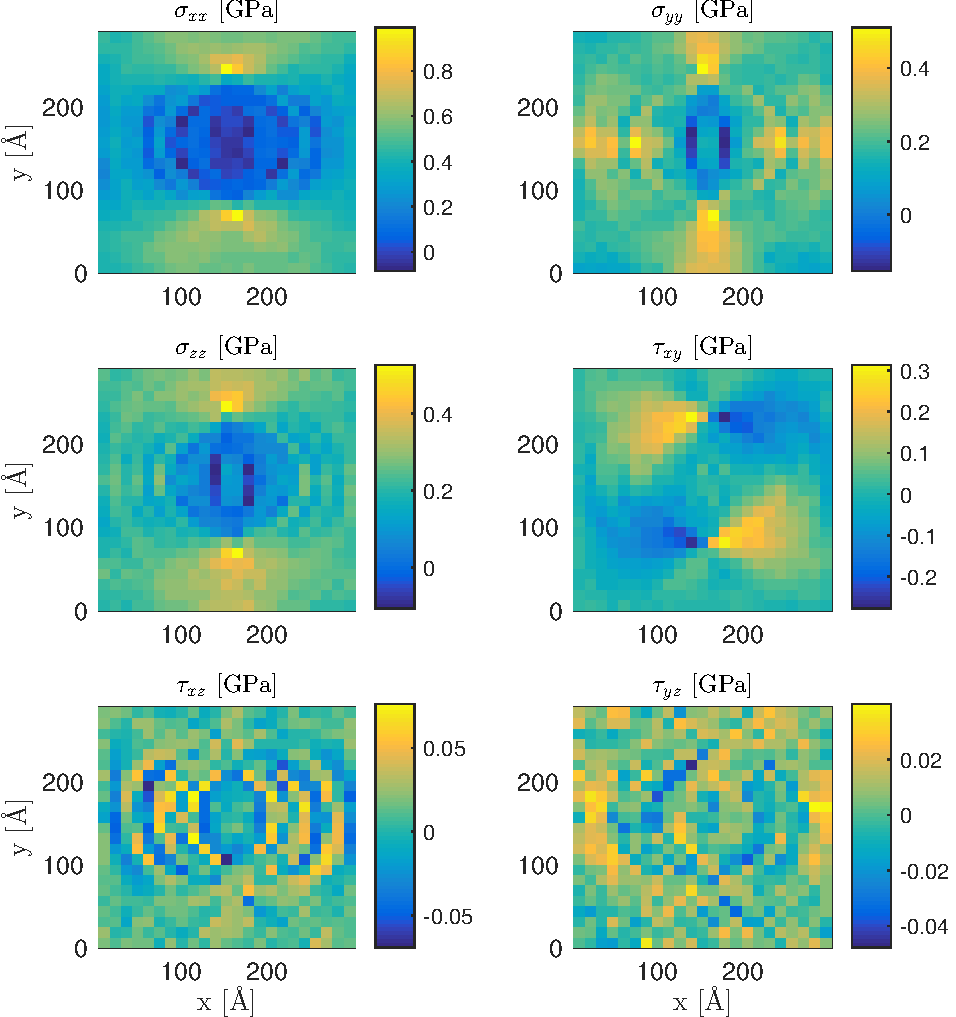
\includegraphics[width=\textwidth]{../figures/thesis/stressfield_snap_propagation_180.pdf}
\caption{Snapshot of stress field during crack propagation. Taken at $t = \SI{180}{\pico\second}$.}
\end{figure}


\begin{figure}
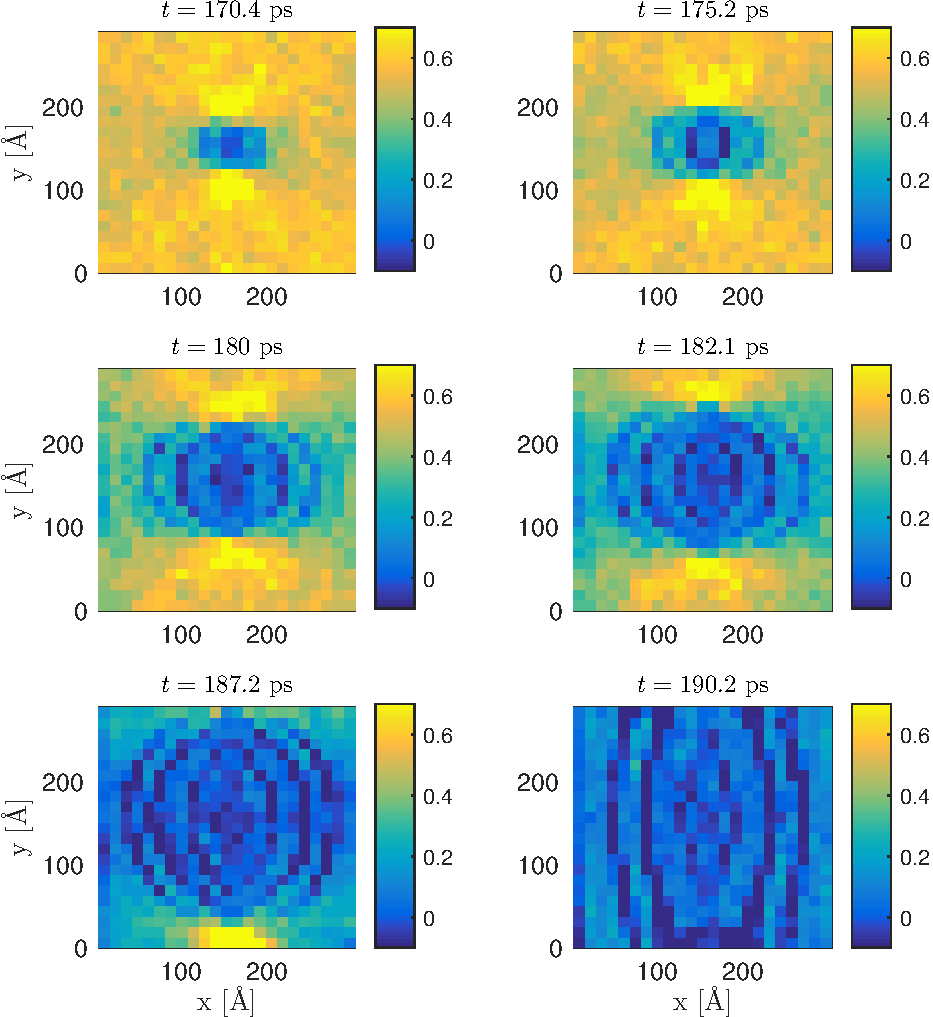
\includegraphics[width=\textwidth]{../figures/thesis/stressfield_timelapse.pdf}
\caption{Timelapse of the stress $\sigma_{xx}$ during crack propagation. There are clear signs of sound waves, and the shape of the waves indicate that the crack is traveling at a speen on the same order of magnitude as the shear wave speed. The color scale is kept equal among the simulations for easier comparison. For that reason, the stress near the crack tip is higher that what is available on the color scale.}
\end{figure}

\begin{figure}
\centering
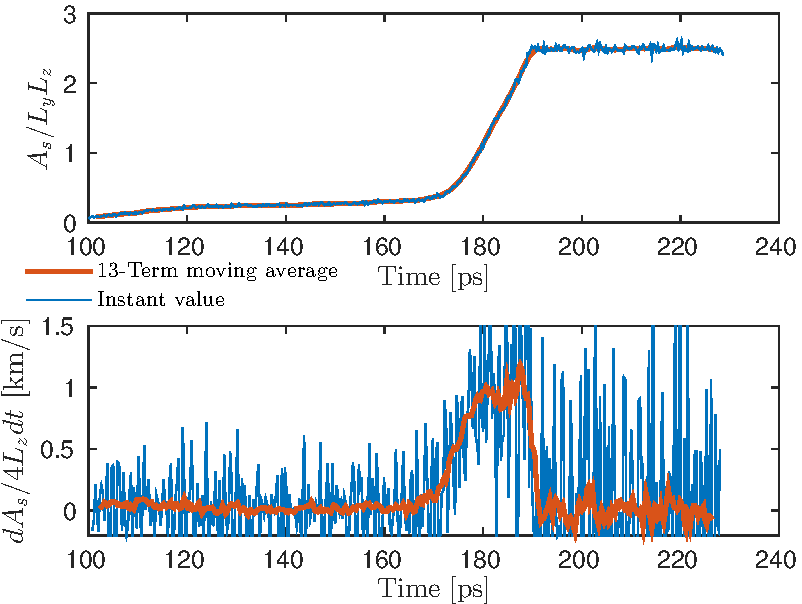
\includegraphics[width=10cm]{../figures/thesis/crack_area_evolution_1048.pdf}
\caption{Crack surface area evolution in time. The upper panel shows the measured area, and the lower panel is an estimate of the crack tip speed. The derivative for the lower panel is calculated using a standard 5-point stencil for the first derivative. The crack surface area was measured useing the Monte Carlo procedure described in section @ref with $N_s = 10^6$, $r_p = \SI{4.0}{\angstrom}$ and $\Delta l = \SI{1.0}{\angstrom}$. }
\end{figure}

\section{A simple characterization of the crack surface: The amount of methane released.}
It might sound farfetched, but I believe that the amount of methane released can be a valuable measure of how the crack surface looks. That is because water molecules either stay on the crack surface, or are immidiately drawn towards the crack surface in a matter of picoseconds. Methane, on the other hand, is free to move in the pore space created by the crack. A first order approach to characterize the crack surface, is therefore to look at how much of the hydrate was dissociated during fracture. A way to estimate this, is to say that the number of cages that are dissociated is the same as the number of free methane molecules in the system.  

\subsection{Estimate by mean squared displacement}
One way of estimating the amount of methane released, is to realize that the motion of the free methane is diffusive. Therefore, the mean square displacement of the methane can be compared to what it would have been if all methane molecules were free to move.

Since the methane gas is purely a Lennard-Jones fluid, literature results for the diffusion coefficient should be readily available. It turns out that this approach is not straightforward. The ...

\paragraph{Problems with this method:}
\begin{itemize}
\item Global oscillations of the system
\item Finite size effects of the diffusivity
\item Quasi-2D
\item Will the method converge?
\item Caculation of the pore volume.
\item The density enters in the literature diffusion constant
\item The conditions for thermal diffusion in the crack might not be present. 
\end{itemize}

\subsection{Estimate by counting}
A more straightforward approach, which is more computationally demanding, is to go through all methane positions, and check wheter they are part of the wall or the void, like what was done when tracking cracks. A particle is considered free if it was part of the void at any time during the simulation. The reason for the ``at any time during the simulation'' is that measuring frame by frame largely underestimates the number of free methanes. Methanes that are free arent necessarily far enough from the closest water molecule to be considered void, but they \emph{are} free to move. To check the that the free methanes are indeed free, the positions of the methanes that were defined as void can be drawn at a point in time after the crack has propagated. @AddFigure

\subsection{Diffusion revisited}
Measuring the number of free methanes using the mean squared displacement turned out to be difficult, but now that the number of free methanes is measured, the diffusion inside the crack can be characterized.
